% This version uses the latex2e styles, not the very ancient 2.09 stuff.
\documentclass{sig-alternate-10pt}
\usepackage{endnotes,url}
%\usepackage{sig-alternate-10pt,endnotes}
\usepackage{epsfig}
\usepackage{amssymb}
\usepackage{amsmath}
\usepackage{lipsum}
\usepackage{algorithm}
\usepackage{algorithmic}
\usepackage{amsfonts}
\usepackage{graphicx}
\usepackage{verbatim}
% Replaced by subfig package
% \usepackage{subfigure}
\usepackage{subfig}
\usepackage{epstopdf}
\usepackage{cite}
\usepackage{array}
\usepackage{multirow}
\usepackage{listings}


\captionsetup[figure]{labelfont={small},textfont={small}}

%\pdfpagewidth 8.5in
%\pdfpageheight 11in
%\baselineskip=12.5pt
%\setlength{\pdfpagewidth}{8.5in}
%\setlength{\pdfpageheight}{11in}
%\usepackage{pdfdraftcopy}

% To import classical math notation used
\input{mathnotation.tex}
% Package for date and time presentation
\usepackage{datetime}
\newcommand{\datation}{\today, \xxivtime}

\def\full{0}        % set 1 for a full tech report version
                    % set 0 for submission version
\def\shownotes{1}   % set 1 for version with author notes
                    % set 0 for no notes
\def\anon{1}        % set 1 to anonymize
                    % set 0 for acks and author names

%%%%%%%  Author Notes %%%%%%%
%
\ifnum\shownotes=1
\newcommand{\authnote}[2]{{ $\ll$\textsf{\footnotesize #1 notes: #2}$\gg$}}
\else
\newcommand{\authnote}[2]{}
\fi
\newcommand{\Anote}[1]{{\authnote{Andrius}{#1}}}

%%%%%%%%%%%%%%%%%%%%%%%%%%%%%%%%%

\newcommand{\namedref}[2]{#1~\ref{#2}}
\newcommand{\tableref}[1]{\namedref{Table}{#1}}
\newcommand{\sectionref}[1]{\namedref{Section}{#1}}
\newcommand{\appendixref}[1]{\namedref{Appendix}{#1}}
\newcommand{\theoremref}[1]{\namedref{Theorem}{#1}}
\newcommand{\remarkref}[1]{\namedref{Remark}{#1}}
\newcommand{\definitionref}[1]{\namedref{Definition}{#1}}
\newcommand{\figureref}[1]{\namedref{Figure}{#1}}
\newcommand{\lemmaref}[1]{\namedref{Lemma}{#1}}
\newcommand{\claimref}[1]{\namedref{Claim}{#1}}
\newcommand{\propositionref}[1]{\namedref{Proposition}{#1}}
\newcommand{\constructionref}[1]{\namedref{Construction}{#1}}
\newcommand{\corollaryref}[1]{\namedref{Corollary}{#1}}
\newcommand{\equationref}[1]{\namedref{Equation}{#1}}
%
\newtheorem{theorem}{Theorem}[section]
\newtheorem{definition}[theorem]{Definition}
\newtheorem{lemma}[theorem]{Lemma}
\newtheorem{claim}[theorem]{Claim}
\newtheorem{obs}[theorem]{Observation}
%


\providecommand{\vs}{vs. }
\providecommand{\ie}{\emph{i.e.,} }
\providecommand{\eg}{\emph{e.g.,} }
\providecommand{\cf}{\emph{cf.,} }
\providecommand{\resp}{\emph{resp.,} }
\providecommand{\etal}{\emph{et al.}}   %Removed trailing space here; usually want non-breaking space with following reference
\providecommand{\etc}{\emph{etc.}}      % No trailing space here either
\providecommand{\mypara}[1]{\smallskip\noindent\emph{#1} }
\providecommand{\myparab}[1]{\smallskip\noindent\textbf{#1} }
\providecommand{\myparasc}[1]{\smallskip\noindent\textsc{#1} }
\providecommand{\para}{\smallskip\noindent}

\newtheorem{axiom}{{\bf  Axiom}}
\newtheorem{defin}{{\bf  Definition}}
\newtheorem{proposition}{Proposition}

\usepackage{enumitem}
\setlist{nolistsep}

%Model parameters

\usepackage[breaklinks=true]{hyperref}
\frenchspacing
\begin{document}

%don't want date printed
\date{}


%make title bold and 14 pt font (Latex default is non-bold, 16 pt)
\title{NoTCP: steganopgraphic tricks to bypass middleboxes}
\ifnum\anon=1
\author{[Paper: \#137]}% \hspace{0.2cm} \ampmtime ]}
\else
\numberofauthors{3}
\author{
\alignauthor Andrius Aucinas\\
\affaddr{University of Cambridge} 
\and
\alignauthor Jon Crowcroft\\
\affaddr{University of Cambridge}
\and
\alignauthor Narseo Vallina-Rodriguez\\
\affaddr{ICSI}
}
\fi
%for single author (just remove % characters)

    
% end author
\maketitle
% Use the following at camera-ready time to suppress page numbers.
% Comment it out when you first submit the paper for review.
%\thispagestyle{empty}
\begin{abstract}
TCP is the de facto transport protocol in the Internet. However it has many limitations that make it ill suited to the modern world of high mobility and multi-homing. Protocol optimizations and filtering performed by middleboxes make extension deployment challenging which has led researchers to explore new ways of exchanging control information between endpoints. In this paper we explore steganographic approaches to smuggle information between endpoints. We design NoTCP -- a mechanism which uses the TCP header fields in combinations that are currently have no defined semantics to hide a small amount of control information from middleboxes and hence bootstrap a control channel. We also present a preliminary study showing how the mechanism works across cellular and WiFi networks.
\end{abstract} 

\section{Introduction}
\label{section:intro}

Extensibility of the Internet has been not like originally envisioned for a long time now, starting with IP layer and extending the \emph{narrow waist} to TCP or even HTTP at large. The problem is caused by the various middleboxes that aim to improve performance\cite{Kopparty:2002ht,Chakravorty:2003dm}, increase security\cite{Handley:2001vp,Vutukuru:2008fc} and solve address shortage problems. Even congestion control has required multiple extensions since protocol's inception and the large number of proposed congestion control schemes~\cite{5462976} suggests that more will be necessary.

In an ideal world all infrastructure is forwards compatible and changes together with the needs of the users. Instead, TCP has become the de facto transport protocol of the Internet and development of its extensions has been very challenging. Proposals including MPTCP~\cite{Handley:vj} for multi-homed endpoints and TCPCrypt~\cite{Mazieres:uz} for ubiquitous end-to-end traffic encryption are necessary for today's networks but deployment has been slow and difficult. Previous work on MPTCP overviews the major problems with different types of middleboxes~\cite{Raiciu:2012ur}.

Although TCP has been built to be extensible via options and reserved bits, all extensions are primarily designed around the limitations of existing network middleboxes\cite{Honda,Guha2005tb,UntoldMiddlebox2011}, but even if options were not filtered, we have run out of the 40-byte TCP option space.

Problems with the size of option space arise in MPTCP when its options are combined with those of regular TCP and therefore needs to change the semantics of a duplicate ACK~\cite{Handley:vj} and there are efforts to define an alternative control stream to work around the limitation of option space~\cite{Bonaventure:wx}. TCPCrypt uses the Data portion of TCP segments to exchange cryptographic keys~\cite{Mazieres:uz}. An alternative way of looking at the problem is to hide the information from the middleboxes as done by steganographic approaches~\cite{Frczek:2012dl,Zielinska:2014fn,Rowland:1997vq,Murdoch:2005fz}.

We propose \emph{noTCP}, an approach complementary to option negotiation which repurposes TCP header fields beyond what is specified. At the same time it is designed to work across most of deployed network infrastructure. At the core of the idea is modification of TCP header fields in a way that is not interfered with by middleboxes or so that such interference can be safely recovered or ignored. The idea builds up from the work on steganography using TCP~\cite{Frczek:2012dl,Murdoch:2005fz}, but we shift the focus from using sequence numbers and options to other fields as well.

With the focus on cellular and WiFi networks due to their renown middlebox peculiarities, we make the following contributions in this work:

\begin{enumerate}
    \item Review the aspects of the TCP protocol that can potentially be used to extend it (Section~\ref{sec:protocolChanges}).
    \item Provide an analysis of current mobile (WiFi and cellular) network behavior in the presence of such modifications (Section~\ref{sec:network}).
    \item Propose a robust method to bootstrap control-stream between two endpoints across middleboxes (Section~\ref{sec:protocol}).
\end{enumerate}

\section{Candidate protocol changes}
\label{sec:protocolChanges}

Without using the options field and only changing the meaning of header fields in a backwards-compatible manner we only have a few options:
\begin{itemize}
    \item Setting header fields to specific values without setting the corresponding flags so they do not have a meaning to legacy implementations.
    \item Assigning one or more of the reserved field bits.
    \item Defining semantics for specific values of currently valid header fields.
\end{itemize}

In this section we overview these different options, discuss their pros and cons and show how real networks interact with them.

\subsubsection*{Unset Flags}
\label{sec:unset}

The only header fields that may or may not have a meaning depending on the corresponding flag are \emph{urgent pointer} and \emph{acknowledgment number}, and the latter is only allowed to be not set for the initial SYN packet.

Urgent pointer is both a good and a bad candidate at the same time: it is already recommended against the use of the urgent mechanism~\cite{Gont:2011vi}, therefore it could be claimed that it is taking up precious space in the TCP header. On the other hand, it is common practice by Network Intrusion Detection Systems (NIDS) to reset the field as it makes it difficult to track the application-layer data~\cite{seolma}. We present our observations of how often the field is filtered in Section~\ref{sec:network}, however although we witnessed the field to be passed through on many of our studied networks and hence it is a usable option, it is not without drawbacks.

Acknowledgment field, on the other hand, is double the length and we saw it successfully pass through the networks in more cases. Nevertheless, unless specific value is signaled out of bound between the two endpoints to use the field with TCP Simultaneous Open, only the initiating end can use it and the responding side needs to acknowledge the understanding of it in some other method. 

\subsubsection*{Reserved bits}

The main difficulty with TCP Reserved bits is that there are only 3 bits unallocated if we consider the three ECN bits added over 10 years ago~\cite{Floyd:up,Ely:uc} but still not universally implemented~\cite{Kuhlewind:2013hr}. Any further reserved bit allocation would therefore be extremely difficult.

Nevertheless, there are proposals that make use of them. One of the proposals for reducing Web latency~\cite{Flach:2013uy} suggests sending multiple copies of packets, but to avoid triggering duplicate acknowledgments add a reserved bit to the header. We confirmed the authors observation that middleboxes do not seem to discard packets with non-compliant TCP flags, however we also saw a number of middleboxes to clear such flags, hence interfering with the duplicate acknowledgment of the proposed scheme. Due to the problem with reserved bit allocation we would recommend using mechanisms we discuss later.

\subsubsection*{Value-specific semantics}

Our remaining class of options, and by far the biggest, is defining protocol semantics based on specific values of certain header fields. It would necessitate generating crafting packets with specific values for initial sequence numbers, window size or a specific checksum value, and we posit that it would be an acceptable choice if such solution is deployable in today's network and can be implemented efficiently.

Initial sequence numbers must be hard to predict as they provide a measure (however weak) of security and until a stronger one (such as TCPCrypt) is universally adopted adding any information to the field in a way that is easily decoded by the receiver weakens security which has been problematic~\cite{Qian:2012bj,Bellovin:uz,Qian:2012wb}.

Window size field is potentially a better candidate, especially if used only during connection setup phase, since data is not typically transmitted during the handshake. We could further claim that even during data exchange a few of the least-significant bits could be sacrificed for carrying other information, however that would prevent flow control from operating properly. Higher-order bits could instead be given up when window scaling option is used to compensate for the decrease of signaled window size, but for every such bit the maximum window would be halved, having negative effects for more capable clients connected though high capacity links. Using the field risks interfering both with TCP flow control mechanism as well as window-size optimizations by the network~\cite{Kopparty:2002ht,Chakravorty:2003dm} performed \eg by Citrix ByteMobile Proxy~\cite{Ha:2006td}. 

There are multiple benefits of using the checksum field. Firstly, it is only used for error detection as opposed to other fields that govern protocol behavior and is either not always necessary due to the layered design of the OSI stack (when error detection is done at the layer below or above), or can be replaced with extensions' separate (MPTCP DSS checksum) or even stronger (TCPCrypt MAC) mechanisms. Secondly, checksum operations are efficient as they only involve one's complement addition. And finally, it is possible to generate checksums in a way that the intended value can recovered by the receiving end after traversing common types of middleboxes that recompute the checksum as we discuss in the following sections.


\section{Methodology}

To test what works on current networks we have developed a simplified implementation of TCP that exchanges packets in the standard order (three-way handshake, data exchange and connection shutdown) but with various header fields modified to our purposes.

The test has been implemented as an Android application and distributed through the \emph{Google Play Store} to collect data from volunteers. The overall structure of the tool is relatively straightforward:
\begin{itemize}
    \item UI which reports aggregated results to the end-users, sends results to the reporting server and manages the overall flow of the tests.
    \item Native implementation of the simplified TCP stack using Raw Unix sockets (\emph{SOCK\_RAW}) to allow us to generate packets at the network layer. This also meant having to drop RST packets generated by the kernel network stack during the test in response to incoming packets associated with connections it is not aware of - packets are delivered to both the raw socket and the kernel network stack.
    \item Server implementation that generates specific answers to incoming packets based on header and payload values.
\end{itemize}

Potential limitations of our methodology include that we do not consider packet resegmentation since the goal is to negotiate any endpoint-specific in packet headers so that correct behavior does not depend on how packets are split or coalesced together. To make sure that it does not happen all our packets contain minimal amount of payload (up to 16 bytes during data exchange) and data exchange only consists of a single message sent each way, in addition to any extra acknowledgments generated by middleboxes. Due to the same reason we also do not take into account congestion control.

Instead of trying to infer which source port number would be assigned to a new connection by the kernel network stack without using it, we randomized the selection within the unprivileged port range. It was a simple optimization that works on any device and minimizes the probability of multiple tests failing due to another application using a particular port. We also repeated the tests on different destination ports, which we discuss in Sec.~\ref{sec:portspec}.

Non-transparent proxies are a major problem for extension deployment, therefore we used another well know and widely deployed tool to detect proxies on our tested networks. The tests were run separately and we used it to discover non-transparent proxies. We primarily use previously developed technique~\cite{Weaver:RHwbx82O} --  non-responsive server test. To see proxying dependence on higher-level protocols we also detect HTTP proxies using techniques proposed in the work, including checking content and header changes, different IP addresses seen for HTTP or non-HTTP traffic, whether non-HTTP traffic on HTTP port is filtered, HTTP traffic is normalized (\ie deliberately modified headers are fixed). Results are presented in Sec.~\ref{sec:proxies}.

\section{Network characteristics}
\label{sec:network}

\begin{table*}[t]
{\small
\begin{center}
\begin{tabular}{| l | >{\centering\arraybackslash}m{1.2cm} | >{\centering\arraybackslash}m{1.6cm} | >{\centering\arraybackslash}m{1.6cm} | >{\centering\arraybackslash}m{1.8cm} | >{\centering\arraybackslash}m{1.6cm} | >{\centering\arraybackslash}m{1.5cm} | >{\centering\arraybackslash}m{1.5cm} | >{\centering\arraybackslash}m{1.5cm} | >{\centering\arraybackslash}m{1.cm} | }
\hline
    \textbf{Net ID} & \textbf{Country} & \textbf{Port-specific} & \textbf{Validate checksum} & \textbf{Drop SYN-ACK data} & \textbf{Normalize SYN Ack number}  & \textbf{Normalize Urgent Pointer} & \textbf{Normalize Reserved} & \textbf{Remap Sequence} \\ \hline \hline
    % Univ Helsinki WiFi
    WiFi edu 1      & Finland               &                        & \checkmark                 &                        &                         &                        &                             &                     \\ \hline
    % Eduroam
    WiFi edu 2      & UK               &                        &                            & \checkmark             &                         & \checkmark             &                             & \checkmark          \\ \hline
    % wgb
    WiFi pub 1      & UK               &                        &                            &                        &                         &                        &                             &                     \\ \hline
    % MKSW germany (carlos)
    WiFi pub 2      & Germany               &                        & \checkmark                 & \checkmark             &                         &                        &                             &                     \\ \hline
    % Virgin home
    WiFi res 1      & UK               &                        & \checkmark                 &                        &                         &                        &                             &                     \\ \hline
    % TEO Lt
    WiFi res 2      & Lithuania               &                        & \checkmark                 & \checkmark             &                         &                        &                             &                     \\ \hline
    % Telefonica Free
    WiFi ent 1      & Spain               &                        & \checkmark                 & \checkmark             &                         &                        &                             &                     \\ \hline
    \hline
    % Finland internet.saunalahti
    Cellular 1      & Finland               &                        &                            &                        &                         &                        &                             &                     \\ \hline
    % GiffGaff
    Cellular 2      & UK               &  443, 993              & -                          & -                      & -                       & -                      & -                           & -                   \\ \hline
    % E-Plus germany
    Cellular 3      & Germany               &                        &                            &                        &                         & \checkmark             &                             & \checkmark          \\ \hline
    % EE/T-Mobile
    Cellular 4      & UK               &               80, 443  & -                          & -                      & -                       & -                      & -                           & -                   \\ \hline
    % Three UK
    Cellular 5      & UK               &                        & \checkmark                 &                        &                         &                        &                             &                     \\ \hline
    % Omnitel LT
    Cellular 6      & Lithuania               &                        & \checkmark                 &                        &                         &                        &                             &                     \\ \hline
\end{tabular}
\end{center}
}
\caption{Network behavior observed through tests generating custom TCP packets. A dash means different cases observed based on port numbers.}
\label{tab:networks}
\end{table*}

We show our collected results in Table~\ref{tab:networks}. Since we were focusing on mobile applications, in our preliminary study we collected results across a few public, residential, university and enterprise WiFi networks as well as 6 cellular networks in 4 different countries: UK, Finland, Germany and Lithuania.

The results include which networks did not filter any modifications (one WiFi and two cellular nets), and which ones discarded packets with invalid checksums, normalized particular fields - either dropped packets or reset to different values - and whether NATs performed only port number remapping or also changed sequence numbers. Only one network provided clients with a global IP (WiFi edu 2).

In traditional NATs~\cite{Egevang:tu} checksum recalculation is very simple: subtract the old header fields from the checksum and add the new ones to minimize the resource use. The networks that deliver packets with invalid checksum only do that as otherwise a packet with invalid checksum would be dropped.

A bigger issue we have discovered is that middleboxes do not always respect the standard and simply drop SYN-ACK packets with payload. We did not see it on cellular networks, but most WiFi (4/7) behaved in such way even though the standard allows handshake packets to contain payload~\cite{Postel:3EDyoxP_,Chu:2011tn}:

\begin{quotation}
    Although these examples do not show connection synchronization using data-carrying segments, this is perfectly legitimate
\end{quotation}

As discussed in Section~\ref{sec:unset}, we can squeeze in a few extra bits of information by defining meaning to header fields when corresponding flags are not set. None of our tested networks filtered Acknowledgment Number field for the initial SYN packet on non-proxied paths and only two networks discarded packets with Urgent Pointer set without URG flag.

Finally we tested interaction reserved header bits. We separated our tests to handshake and data exchange parts as well as set each bit individually, however we did not observe different behavior for these: all reserved bits were either allowed through or cleared at both phases. Importantly, we did not observe cases when such packets are dropped.


\subsection{Port-specific middlebox behavior}
\label{sec:portspec}

We repeat our tests on a few ports:
\begin{itemize}
    \item 80, 443 - HTTP and HTTPS
    \item 993 - Secure IMAP port
    \item 5228 - Google cloud messaging port
    \item 6969 - random port number
    \item 8000 - common HTTP proxy port number
\end{itemize}

We only observed port-specific behavior on two networks: \emph{Cellular 2} and \emph{Cellular 4}. In the first case, traffic travels over SSL ports (443, 993) unmodified except for packets with invalid checksum being dropped. Our traffic was not encrypted and an increasing proportion of traffic is served over SSL. A commercially deployed HTTP accelerator reports the proportion of HTTPS requests to be close to that of HTTP\footnote{\url{http://db.awazza.com/users/global/}}, making the value of such proxying questionable.

We confirmed the middlebox to be a ByteMobile proxy. It replaces the original connections with a new one which adds options not present in original packets, changes window size and resets other fields to new values to optimize TCP for cellular networks~\cite{Ha:2006td}. Such behavior makes deployment of any protocol modifications or extensions very difficult (e.g. we verified that TCPCrypt does not work on this network). Although we did not see more cases of it, the company claims over 160 clients.

In the second case, traffic was only modified when going to ports 80 and 443. As we discuss below, the network optimizes HTTP traffic and since our traffic does not resemble valid HTTP, it is dropped.

\subsection{Non-transparent proxies}
\label{sec:proxies}

Since proxies make new changes very difficult, we checked for non-transparent oes on in our tested networks on a number of popular port numbers:
21, 22, 25, 80, 110, 135, 139, 143, 161, 443, 445, 465, 585, 587, 993, 995, 1194, 1723, 5060, 6881, 9001.

\begin{table}[t!]
{\small
\begin{center}
\begin{tabular}{| l | >{\centering\arraybackslash}m{1.8cm} | >{\centering\arraybackslash}m{3.7cm} |}
\hline
    \textbf{Net ID} & \textbf{Radio Technology} & \textbf{Proxied Ports} \\ \hline \hline
    Cellular 2      & HSPA                      & 21, 22, 25, 80, 110, 135, 143, 161, 465, 585, 587, 995, 1194, 1723, 5060, 6881, 9001 \\ \hline
    Cellular 4      & GPRS                      & 80, 110, 143 \\ \hline
    Cellular 4      & HSPA                      & 80, 110, 143 \\ \hline
    Cellular 4      & LTE                       & 80, 110, 143, 443, 993, 995 \\ \hline
    % T-Mobile, part of EE
    Cellular 4*     & HSPA                     & 25, 80, 110, 143 \\ \hline
    % Virgin on T-Mobile
    Cellular 4**    & HSPA                    & 25, 80, 110, 143 \\ \hline
\end{tabular}
\end{center}
}
\caption{Non-transparent proxies and proxied port numbers by radio technology}
\label{tab:proxies}
\end{table}

Results are summarized in Table~\ref{tab:proxies}. Cellular 2 proxies almost all of our tested ports except for 443 and 993 as observed before. 
Cellular 4 shows non-uniform behavior across the network. It is not obvious why ports commonly used for encrypted communication are proxied over LTE, we only recorded 1 case for HTTPS. The other two cases (* and **) seem related to the operator being formed from two merged operators. These differences are evident in \emph{whois} records, device-reported network name (\textbf{*} shows the old operator name) and MVNO setup (\textbf{**} setup with the old operator).

It is not safe to estimate proxying just from \emph{whois} records: they do not necessarily match the operator names and we saw the same address ranges used with all device-reported network names for HSPA and LTE radios. An active test is needed reliably detect proxies.

Proxying is protocol-dependent in some cases: looking at port 80, Cellular 4\*\* modified HTTP headers, performed transcoding and reordered header fields, but only modified non-HTTP traffic for one of the two sessions. On Cellular 1 (15 sessions) two sessions show DNS proxies and on Cellular 5 (47 sessions) in two cases non-HTTP traffic is filtered on port 80, signaling that there still may be some proxying within the networks. Finally, Cellular 2 and 4 both reorder HTTP headers and perform transcoding, but Cellular 4 does not always allow non-HTTP traffic. We did not have data about Cellular 6, but results discussed above suggest that there are no non-transparent proxies present.

All other networks did not show non-transparent proxy behavior, but the ones who did pose a challenge that is not easily solved. Proxies potentially change every aspect of the original connection and hiding any information within the packet becomes extremely difficult since any value that a proxy does not recognize is reset.


%    an_op_name    | an_cell_net_type | an_country | port |    ip_global (simplified to network address. Included the owner according to whois
% db)
% -----------------+------------------+------------+------+-----------------
%  EE              | GPRS             | gb         |   80 | 31.72/19 (EE)
%  EE              | GPRS             | gb         |  110 | 31.72/19 (EE)
%  EE              | GPRS             | gb         |  143 | 31.72/19 (EE) 
%  EE              | HSPA             | gb         |   25 | 31.96/21 (EE), 149.254/16 (T-Mobile UK), 178.96/12 (EE)
%  EE              | HSPA             | gb         |   80 | 31.80/21 (EE), 31.96/21 (EE), 149.254/16 (T-Mobile UK), 178.96/12 (EE), 213.205.224/12 (EE)
%  EE              | HSPA             | gb         |  110 | 31.80/21 (EE), 31.96/21 (EE), 149.254/16 (T-Mobile UK), 178.96/12 (EE), 213.205.224/12 (EE)
%  EE              | HSPA             | gb         |  143 | 31.80/21 (EE), 31.96/21 (EE), 149.254/16 (T-Mobile UK), 178.96/12 (EE), 213.205.224/12 (EE)
%  EE              | LTE              | gb         |   80 | 31.96/21 (EE), 89.192/16 (EE), 213.205.224/12 (EE)
%  EE              | LTE              | gb         |  110 | 31.96/21 (EE), 89.192/16 (EE), 213.205.224/12 (EE)
%  EE              | LTE              | gb         |  143 | 31.96/21 (EE), 89.192/16 (EE), 213.205.224/12 (EE)
%  EE              | LTE              | gb         |  443 | 213.205.224/12 (EE)
%  EE              | LTE              | gb         |  993 | 31.96/21 (EE), 89.192/16 (EE), 213.205.224/12 (EE)
%  EE              | LTE              | gb         |  995 | 31.96/21 (EE), 89.192/16 (EE), 213.205.224/12 (EE)
%  T-Mobile        | HSPA             | gb         |   25 | 31.96/21 (EE), 149.254/16 (T-Mobile)
%  T-Mobile        | HSPA             | gb         |   80 | 31.96/21 (EE), 149.254/16 (T-Mobile)
%  T-Mobile        | HSPA             | gb         |  110 | 31.96/21 (EE), 149.254/16 (T-Mobile)
%  T-Mobile        | HSPA             | gb         |  143 | 31.96/21 (EE), 149.254/16 (T-Mobile)
%  Virgin          | HSPA             | gb         |   25 | 149.254/16 (T-Mobile)
%  Virgin          | HSPA             | gb         |   80 | 149.254/16 (T-Mobile)
%  Virgin          | HSPA             | gb         |  110 | 149.254/16 (T-Mobile)
%  Virgin          | HSPA             | gb         |  143 | 149.254/16 (T-Mobile)
%  giffgaff        | HSPA             | gb         |   21 | 82.132/16 (O2)
%  giffgaff        | HSPA             | gb         |   22 | 82.132/16 (O2)
%  giffgaff        | HSPA             | gb         |   25 | 82.132/16 (O2)
%  giffgaff        | HSPA             | gb         |   80 | 82.132/16 (O2)
%  giffgaff        | HSPA             | gb         |  110 | 82.132/16 (O2)
%  giffgaff        | HSPA             | gb         |  135 | 82.132/16 (O2)
%  giffgaff        | HSPA             | gb         |  143 | 82.132/16 (O2)
%  giffgaff        | HSPA             | gb         |  161 | 82.132/16 (O2)
%  giffgaff        | HSPA             | gb         |  465 | 82.132/16 (O2)
%  giffgaff        | HSPA             | gb         |  585 | 82.132/16 (O2)
%  giffgaff        | HSPA             | gb         |  587 | 82.132/16 (O2)
%  giffgaff        | HSPA             | gb         |  995 | 82.132/16 (O2)
%  giffgaff        | HSPA             | gb         | 1194 | 82.132/16 (O2)
%  giffgaff        | HSPA             | gb         | 1723 | 82.132/16 (O2)
%  giffgaff        | HSPA             | gb         | 5060 | 82.132/16 (O2)
%  giffgaff        | HSPA             | gb         | 6881 | 82.132/16 (O2)
%  giffgaff        | HSPA             | gb         | 9001 | 82.132/16 (O2)


\section{Protocol negotiation}
\label{sec:protocol}

What is common to all candidate protocol changes described above is that they are very limited in size and therefore sufficient to exchange an opcode or an ID. Other protocol details must instead be exchanged either out of band, implicit to the opcode, or explicitly by redefining the meaning of part of the data payload or previously exchanged information.

\subsection{Opcode embedding}

\begin{figure}[t!]
\centering
\small{
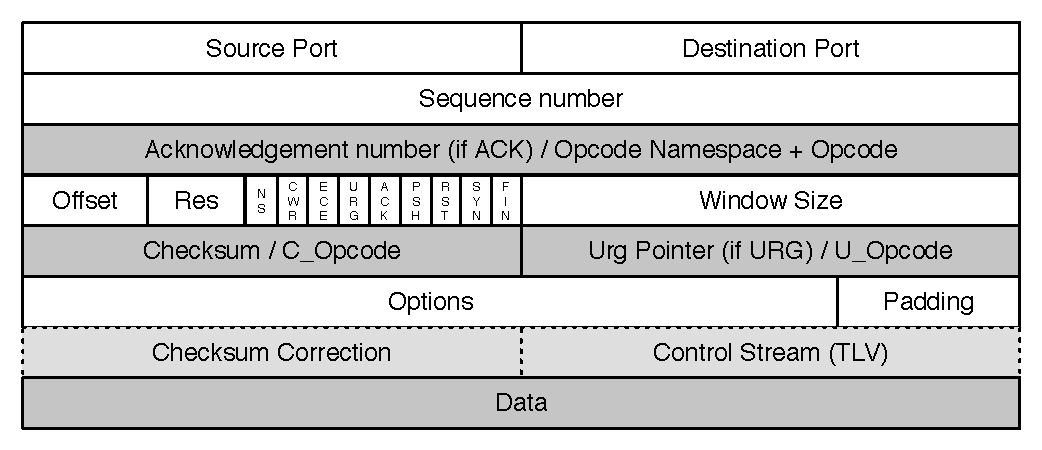
\includegraphics[width=\columnwidth]{figs/tcp-header}
% \vspace{-2mm}
\caption{NoTCP Header with overloaded fields and extra Checksum Correction / Control Stream fields within payload}
\label{fig:header}
}
% \vspace{-4mm}
\end{figure}

A surprising result in our tests is that the \emph{Acknowledgment Number} field without the ACK flag set is passed on all non-proxied connections. In addition, it is a 32-bit value and we can allocate part of it (\eg 8 or 16 bits) to signal that the rest of the field is significant. The exact allocation is subject to further discussion, but we suggest using the first 16 bits as \emph{Extension Space} and the others as $Opcode$ (Fig.~\ref{fig:header}), carrying the desired opcode. For simultaneous open we can use the same mechanism in both directions.

For acknowledging extensions in SYN-ACK packet we use Urgent Pointer and Checksum fields. Our tests indicate that neither choice is guaranteed to succeed, therefore we combine the two by redefining their values when SYN=1. We define Urgent Pointer to be $Opcode_U$ when URG=0 and Checksum to carry a meaning when Urgent Pointer = 0 to get around the cases where one is blocked but the other one is not. Across all networks we have tested in our preliminary study at least one of the choices succeeds.

Checksum value can not be used directly as an opcode since it changes at every level of NAT. The traditional NAT does a simple recalculation of the checksum~\cite{Egevang:tu}: subtracts the original source address and port number (in some cases also the sequence number) and adds the new values. The received Checksum after \(n\) NAT hops is therefore
\vspace{-2mm}
\begin{align*}
Checksum_2 & = Checksum_1 - src_1 + src_2 \\
Checksum_i & = Checksum_{i-1} - src_{i-1} + src_i \\
 ... \\
Checksum_n & = Checksum_1 - src_1 + src_n
\end{align*}
\vspace{-2mm}

We encode the Opcode as a target checksum so that it is recoverable by a simple binary subtraction of source port number, address and sequence numbers in case they are remapped by the NAT (3-7 16-bit operations in total): 
\vspace{-2mm}
\begin{align*}
Checksum_{target} & = Opcode + src_1 \\
Checksum_n = Opcode_C & = Opcode + src_n
\end{align*}
\vspace{-2mm}

There are two choices for setting checksum to a specific value: invalid checksum or adding padding payload. The latter can only be done when the receiving end is already expecting it, since it should not pass such payload up to the layer above, but keeps a packet valid from network's perspective.

For our prototype we assign the first 16 bits of the payload as \emph{Checksum Correction} to force a specific checksum, in line with other extensions which reuse part of data payload for option negotiation and maintaining validity of a packet. This Checksum Correction field is not delivered to the application. TLV-Encoded (Type-Length-Value) Control Stream can be present in data part~\cite{Bonaventure:wx} of the SYN-ACK packet after the Checksum Correction field.

Sending data with SYN-ACK packet works on all cellular networks we have tested, but does not on most WiFi. However, for all three cases (Urgent pointer and checksum) the information either reaches the destination as intended, or the packet is dropped. On all of our tested networks at least one case succeeds if there is no non-transparent proxy.

\subsection{Bootstrapping control stream}

We use the embedded opcodes in the handshake to exchange sufficient control information to bootstrap a complete control stream. We extend the three-way handshake with fields shown in Fig.~\ref{fig:header}:

\begin{enumerate}
\item \textbf{SYN}: the active opener sends SYN packet with \emph{$Opcode Namespace$ + $Opcode$} and ACK unset.
\item \textbf{SYN-ACK}: if passive opener recognizes the namespace and the $Opcode$, it replies with SYN-ACK with $Opcode_U$ = $Opcode$ (URG unset) to acknowledge the Opcode.
\item If passive opener does not receive an ACK, retransmit with $Opcode_C$ and \emph{Checksum Correction}. If that fails as well, retransmit SYN-ACK with an invalid checksum. Finally, fall back to vanilla TCP and retransmit a standard SYN-ACK.
\item \textbf{ACK}: when active opener receives a packet, it checks for $Opcode_U$ (if URG is unset). Otherwise, it checks if Checksum = $Opcode_C$ as described above. If no Opcode is recoverable, fall back to vanilla TCP and transmit a standard ACK.
\item Otherwise both openers recognize the $Opcode$. Active opener sends an ACK packet with TLV-encoded control information in packet payload. The control stream has been successfully bootstrapped.
\end{enumerate}

\begin{figure}[t!]
\centering
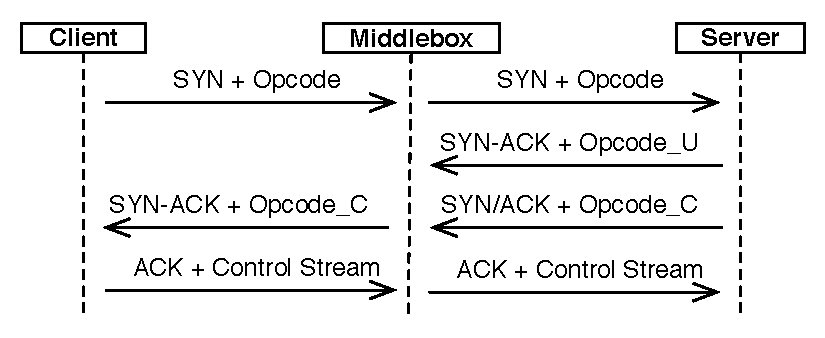
\includegraphics[width=.9\columnwidth]{figs/handshake}
% \vspace{-2mm}
\caption{Example handshake with extension negotiation}
\label{fig:handshake}
% \vspace{-4mm}
\end{figure}

An example handshake is shown in Fig.~\ref{fig:handshake}. In this case a client (active opener) sends a SYN packet as show above. The packet traverses a middlebox which does not remove the opcode and reaches the Server (passive opener). The Server replies with SYN-ACK with U\_Opcode which is discarded by the middlebox. It then retransmits SYN-ACK with $Opcode_C$ and Checksum Correction bits, which reaches the Client. The client recovers and verifies the received opcode. Both endpoints are now assumed to understand the meaning of the opcode, therefore the client replies with an ACK with control information acknowledging reception of the $Opcode$ from the Server.

An issue with putting control stream into packet payload is that some middleboxes split ACK packets with data into two: one only acknowledging the received data and the other one with the actual payload. It is not an issue with TLV-encoded control stream in the payload, because it will be delivered to the receiver first. Hence if the passive opener receives data during or immediately after the handshake but can not decode that as valid TLV-encoded control information, it treats that as application data and falls back to vanilla TCP.

After the first data packets there are potential problems with segment splitting and coalescing : control stream may reach the destination in the middle of a payload of a packet and would be impossible to find without scanning the whole payload. Either SCTP style chunking or MPTCP DSS option can be reused to get around the problem. The obvious drawback of such choice is that control stream becomes subject to flow control. We leave refinement of the full control channel for future work.

\section{Discussion}

The main points of discussion on \emph{NoTCP} are the same as with all TCP extensions: is it necessary, is it deployable and is it forwards-compatible? We have discussed the first two throughout the paper, but the biggest challenge for forwards-compatibility is NoTCP's overloading of header fields instead of using options. It is an extremely hard sell for standards bodies. However the main motivation of our work is precisely that options are no longer a usable choice for new extensions hence such position is justified.

The exact protocol semantics are subject to further testing and discussions. The main goal of this work is to identify potential methods for exchanging control information by hiding it from existing middleboxes and we show how a full control stream for TCP can be bootstrapped by overloading the meaning of underspecified header fields.

We also need to extend our study to more networks to make sure that our proposed method of exchanging control information works in diverse scenarios. More importantly, we have left open the question of finding a method to hide such information from non-transparent proxies. The easiest albeit very limited solution is to identify and cache port numbers that allow unmodified traffic. Our goal instead is to study commonly found proxy implementations in detail in order to quickly identify them as well as encode information within their own operating patterns.

\section{Related Work}
\label{sec:related}

Steganography has been used in the past to hide information within network protocols. The main focus has been on covert channels that violate system's security policy and initial sequence numbers~\cite{Rowland:1997vq}, TCP Timestamps~\cite{Giffin:2002wh} and combinations with IP flags~\cite{Murdoch:2005fz}. There are detection techniques for these methods and our main goal is to exchange a small amount of control information rather than a genuine covert channel, asking for a different design.

TCP implements an \emph{urgent mechanism} at its core that allows the sending user to stimulate the receiving user to accept some \emph{urgent data}. The mechanism is often quoted as providing ``out-of-bound'' data delivery even though it is specified that it is not a mechanism for sending such data. Furthermore, there are ambiguities regarding the semantics of the urgent pointer, Network Intrusion Detection Systems (NIDS) tend to clear the URG flag and pointer and in general it is recommended against the use of the mechanism~\cite{Gont:2011vi}.

AccECN proposal~\cite{Kuhlewind:2014vd} uses an additional reserved bit, overloads the meaning of already assigned ECN~\cite{Floyd:up} and NS~\cite{Ely:uc} bits and redefines Urgent Pointer as Non-Urgent when URG is not set. The idea is highly related to ours, but reserving the field solely for ECN use prevents other extensions from using. Furthermore, we saw that some networks block packets with such field, making it especially difficult to use for ECN.

Generic control stream for MPTCP~\cite{Bonaventure:wx} can be reused once it has been negotiated. It proposes mapping such stream into a separate sequence number space and exchange control data over established subflows, only modifying the MPTCP DSS option to differentiate control and data streams. The underlying assumption, however, is that MPTCP is already deployed and that existing deployments will be forwards-compatible with the new specification.

%More generally SCTP uses \emph{data chunks} to differentiate between different subflows. Each packet can contain multiple TLV-encoded chunks to separate user data and control information. Despite its challenged deployment in the Internet, SCTP over DTLS is being used as the basis of WebRTC data protocol~\cite{Tuexen:wv} and we suggest that such chunking could be used on top of \emph{noTCP} once control channel has been bootstrapped.


\section{Conclusion}
TBD
%\input{conclusion}

\ifnum\anon=0
\subsection*{Acknowledgments}

\fi


% \clearpage
%Only show things we really cite :)
% \nocite{*}
{

\bibliographystyle{abbrv}
\small 
\bibliography{references}
}

%\appendix 
%\input{data}

\end{document}







